\subsection{Входные сигналы (воздействия на цепь) и их математическое описание во временной и частотной областях}


Синусоидальный ток - ток, изменяющий свое значение во времени по синусоидальному закону.

%Спасибо, Капитан Очевидность

\begin{equation}
I = I_m \sin(\frac{2 \pi }{T} t + \psi) = I_m \sin ( \omega t + \psi )
\end{equation}

Где:

\begin{itemize}
\item
$ I_m $  - амплитуда
\item
$ T $ - период
\item
$ \psi $ - сдвиг по фазе
\end{itemize}


Синал так же может быть представлен в комплексной форме. см. ~(\S \ref{sec:complex})

На частотной диаграмме такое отображается как вращающийся вектор.

%какие сиглалы, какое временное описание, как сделать преобразование лапласа, не обязательно синусоида.


Сигналы сложной формы могут быть разложены к ряд Фурье, тогда их математическое описание будет представлять собой сумму гармонических колебаний, с которыми можно работать стандартными методами, затем применяя метод наложения.

\begin{center}
	\begin{figure}[h!]
		\center{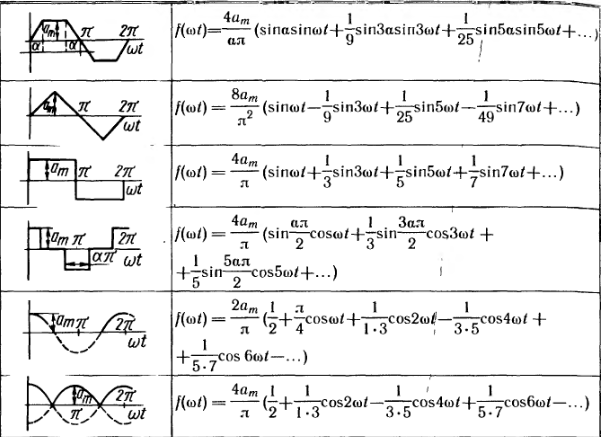
\includegraphics[scale=0.7]{table_fuuurie.png}}
		\caption{Пример метода переменных состояния}	
	\end{figure}
\end{center}



\pagebreak